% Generated by src/build_artifacts.py; source: results/revision-v2/*.json
\begin{figure}[t]
\centering
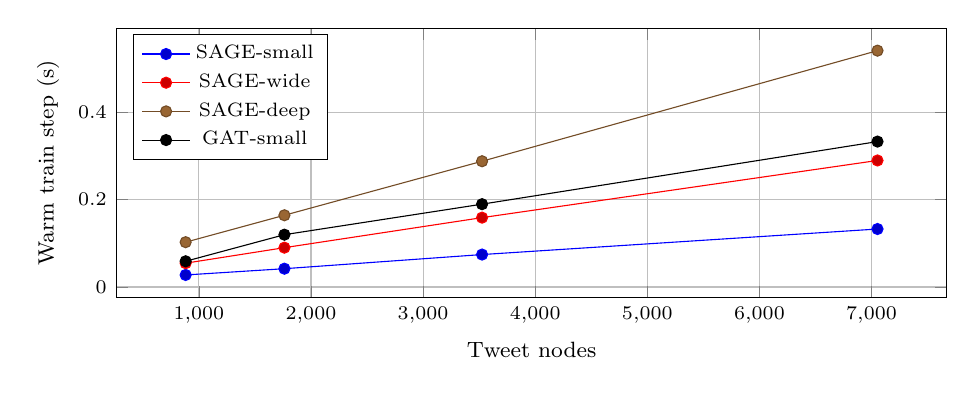
\begin{tikzpicture}
\begin{axis}[width=\columnwidth,height=5cm,xlabel={Tweet nodes},ylabel={Warm train step (s)},
legend style={font=\scriptsize,at={(0.02,0.98)},anchor=north west},
tick label style={font=\scriptsize},label style={font=\footnotesize},grid=major]
\addplot+[mark=*] coordinates {(882,0.02757) (1763,0.04193) (3526,0.07431) (7053,0.13278)};
\addlegendentry{SAGE-small}
\addplot+[mark=*] coordinates {(882,0.05455) (1763,0.09009) (3526,0.15886) (7053,0.28978)};
\addlegendentry{SAGE-wide}
\addplot+[mark=*] coordinates {(882,0.10265) (1763,0.16430) (3526,0.28799) (7053,0.54124)};
\addlegendentry{SAGE-deep}
\addplot+[mark=*] coordinates {(882,0.05893) (1763,0.11981) (3526,0.18970) (7053,0.33301)};
\addlegendentry{GAT-small}
\end{axis}
\end{tikzpicture}
\caption{Measured optimizer-step scaling on nested real tweet subgraphs plus their account neighbors. No synthetic tweets are added.}
\label{fig:scaling}
\end{figure}
